%-------------------------------------------------------------------------------
\section{Findings}
%-------------------------------------------------------------------------------

To compare the  modified autofz with the proposed autofz, we tested it against the 
targets: exiv2, nm, mojs, and tcpdump. Initial test indicate that the ARM64 compatible 
autofz performs similarly to the unmodified autofz. Figure \ref{fig:exiv2_compare_orig_arm64} 
displays bitmap density covered of the individual algorithms in our ARM64 implementation, 
as compared to a similar plot from Fu et. al\cite{fu_autofz_2023}.

\begin{figure}
    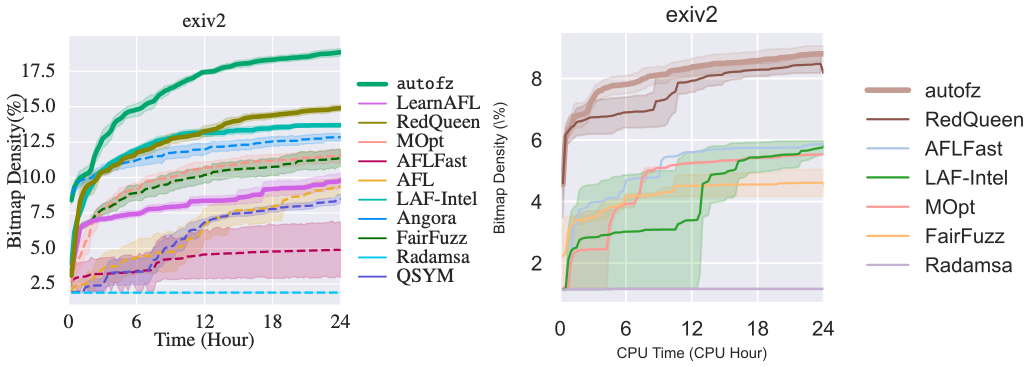
\includegraphics[width=0.52\textwidth]{figs/exiv2_compare_orig_arm64.png}
    \centering
    \caption{A comparison of bitmap density covered in the original\cite{fu_autofz_2023} and our 
    coverage during initial fuzzing of exiv2}
    \label{fig:exiv2_compare_orig_arm64}
\end{figure}

Bitmap density coverage of our initial fuzzing campaign against tcpdump is plotted 
in figure \ref{fig:tcpdump_bmdensity_8Mar2024}, shown as a comparison with results 
from Fu et al.\cite{fu_autofz_2023}.

\begin{figure}
    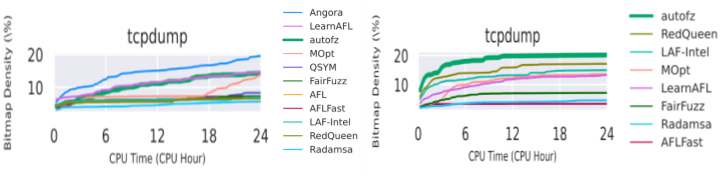
\includegraphics[width=0.52\textwidth]{figs/tcp_compare_orig_arm64.png}
    \centering
    \caption{A comparison of bitmap density covered in the original\cite{fu_autofz_2023} and our 
    coverage during initial fuzzing of tcpdump}
    \label{fig:exiv2_compare_orig_arm64}
\end{figure}

In addition to producing an ARM64 compatible autofz, we identified a potential improvement for autofz.
Existing versions of autofz use bitmap coverage to rank fuzzers during the preparation, but bitmap
coverage may not be the best metric for identifying the most effective fuzzers for a target. While
bitmap coverage indicates the portion of a target that was fuzzed, it does not guarantee bug discovery.
To resolve these problems, we plan to modify autofz, so fuzzers that discover more bugs during the
preparation phase are rewarded with more resources during the focus phase because discovering more bugs
across a smaller area of code decreases the attack surface by more entry points than discovering fewer
bugs over a greater area of the code.